%This code was made by (c)Liudmila Chizhikova for Moscow Aviation Institute journal "Trudy MAI"
%October 2021
%Copyright (c) 2021 Liudmila Chizhikova. 
%Initiative work of LLC Laboratory SARDA. All rights reserved
%This file is subject to the Creative Commons CC BY 4.0

%%%%%%%%%%%%%%%%%%%%%%%%%%%%%%%%%%%%%%%%%%%%%%%%%%%%%%%%%%%%%%%%%%%%%%%%%%%%
% Основная часть статьи на русском языке
%                           
\section*{ Введение}
\par Напишите здесь введение к своей статье

Пример математической формулы в тексте:
\begin{equation}
    y = x^2
\end{equation}

Пример ссылки на источник \cite{b2} Ссылка на источник 1 \cite{b1}
Пример ссылки на таблицу: Таблица \ref{tab:my_label} %ссылка на номер таблицы
\section*{ Методы исследования}
\par Опишите методы исследования, с помощью которых были получены результаты
\subsection*{Теоретические методы}
Опишите теоретические методы исследования (если они были)
\subsection*{Эмпирические методы}
Опишите свой эксперимент (если проводился)

\section*{Результаты}
Опишите результаты исследования.

\section*{Заключение}
Напишите заключение к работе, основные выводы
\clearpage
%%%%%%%%%%%%%%%%%%%%%%%%%%%%%%%%%%%%%%%%%%%%%%%%%%%%%%%%%%%%%%%%%%%%%%%%%%%%%%%%%%%%%%
% Примеры использования и вставки таблиц, формул
%%%%%%%%%%%%%%%%%%%%%%%%%%%%%%%%%%%%%%%%%%%%%%%%%%%%%%%%%%%%%%%%%%%%%%%%%%%%%%%%%%%%%%%
%
\selectlanguage{russian}
\section{Примеры}

%Математические формулы следует набирать внутри блока equation
\begingroup
\subsection{Математические формулы}
\begin{equation}
y = 2x^1+5;
\end{equation}
\begin{equation}
%Греческие буквы следует набирать как
a = \alpha    
\end{equation}

\begin{equation}
    \gamma +\rho = \sigma 
    \delta = \epsilon
\end{equation}
\endgroup
%\newline

%%%%%%%%%%%%%%%%%%%%%%%%%%%%%%%%%%%%%%%%%%%%%%%%%%%%%%%%%%%%%%%%%%%%%%%%%%%%%%%%%%%%%%
\begingroup
\subsection{Таблицы}
%Таблицы следует набирать внутри блока
\begin{table}
    \centering
    \begin{tabular}{c|c|c}
        Название столбца 1 & Название столбца 2& еще столбец \\
        \hline
        Данные столбца 1 & Данные столбца 2& 
    \end{tabular}
    \caption{Название таблицы}
    \label{tab:my_label}
\end{table}
\endgroup
%%%%%%%%%%%%%%%%%%%%%%%%%%%%%%%%%%%%%%%%%%%%%%%%%%%%%%%%%%%%%%%%%%%%%%%%%%%%%%%%%%%%%%
%Рисунки и схемы следует набирать внутри блока, предварительно загрузив графический файл в проект
\begingroup
\subsection{Рисунки}
\begin{figure}
  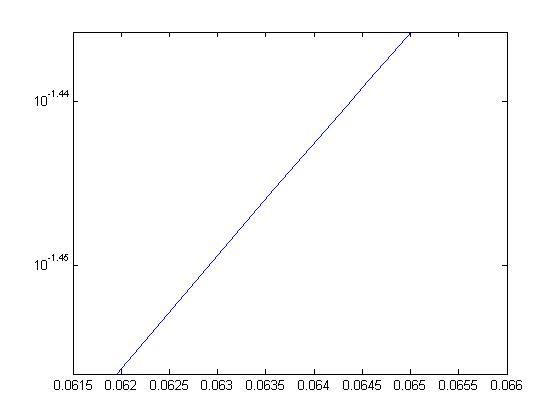
\includegraphics[width=\textwidth]{Scheme_example.jpg} %Название файла рисунка
    %Добавьте здесь свое название рисунка, схемы
   \caption{Математическая зависимость}
    \label{fig:my_label}
\end{figure}
\endgroup






